
\chapter[Dạng bài: Quãng đường của vật\\ dao động điều hòa;\\Dạng bài: Thời gian của vật\\ dao động điều hòa]{Dạng bài: Quãng đường của vật dao động điều hòa;\\Dạng bài: Thời gian của vật dao động điều hòa}
\section{Lý thuyết}
\subsection{Quãng đường của vật dao động điều hòa}
\begin{itemize}
	\item Quãng đường vật đi được trong 1 chu kì:
	\begin{equation*}
		s=4A.
	\end{equation*}
	\item Quãng đường vật đi được trong $1/2$ chu kì:
	\begin{equation*}
		s=2A.
	\end{equation*}
	\item Quãng đường vật đi được từ VTCB ra biên và ngược lại (trong $\dfrac{T}{4}$):
	\begin{equation*}
		s=A.
	\end{equation*}
	
	Với $A$ là biên độ dao động.
\end{itemize}
\subsection{Mối liên hệ giữa dao động điều hòa và chuyển động tròn đều}

Khi vật dao động điều hoà từ $x_1$ đến $x_2$ thì tương ứng với vật chuyển động tròn đều từ M đến N với $x_1$, $x_2$ lần lượt là hình chiếu của M và N lên $\text{O}x$.
\begin{center}
	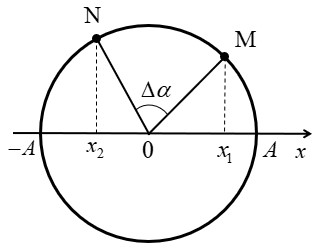
\includegraphics[scale=0.8]{../figs/VN12-PH-02-A-001-7-V2-1.jpg}
\end{center}
Thời gian ngắn nhất vật dao động đi từ $x_1$ đến $x_2$ bằng thời gian vật chuyển động tròn đều từ M đến N.
\begin{equation*}
	t_\text{MN}=\Delta t=\dfrac{\Delta\alpha}{\omega}.
\end{equation*}
\subsection{Thời gian của vật trong dao động điều hòa}
\begin{center}
	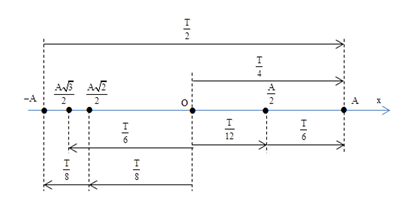
\includegraphics[scale=1.1]{../figs/VN12-PH-02-A-001-4-V2-2}
\end{center}
\section{Mục tiêu bài học - Ví dụ minh họa}
\begin{dang}{Sử dụng được phương trình dao động\\ và đường tròn lượng giác để xác định\\ quãng đường đi được}
	\viduii{3}{Một vật dao động điều hòa với phương trình $x=4\cos\left(2\pi t+\dfrac{\pi}{3}\right)$ ($x$ tính bằng cm, $t$ tính bằng s). Quãng đường mà vật đi được trong thời gian $\SI{3}{\second}$ là
		\begin{mcq}(4)
			\item $\SI{48}{\centi\meter}$.
			\item $\SI{15}{\centi\meter}$.
			\item $\SI{56}{\centi\meter}$.
			\item $\SI{32}{\centi\meter}$.
		\end{mcq} 
	}
	{\begin{center}
			\textbf{Hướng dẫn giải}
		\end{center}
		
		Chu kì dao động của vật là
		\begin{equation*}
			T=\dfrac{2\pi}{\omega}=\dfrac{2\pi}{2\pi\,\text{rad/s}}=\SI{1}{\second}.
		\end{equation*}
		
		Phân tích khoảng thời gian $\SI{3}{\second}$
		\begin{equation*}
			\SI{3}{\second}=3T.
		\end{equation*}
		
		Vì quãng đường vật đi được trong $1T$ là $4A$ nên quãng đường mà vật đi được trong thời gian $\SI{3}{\second}$ là
		\begin{equation*}
			S=3\cdot4A=12A=12\cdot\SI{4}{\centi\meter}=\SI{48}{\centi\meter}.
		\end{equation*}
		
		\textbf{Đáp án: A.}
	}
	\viduii{3}{Một vật dao động điều hòa với phương trình $x=7\cos\left(2\pi t-\dfrac{\pi}{3}\right)$ ($x$ tính bằng cm, $t$ tính bằng s). Quãng đường mà vật đi được trong thời gian $\SI{5,5}{\second}$ là
		\begin{mcq}(4)
			\item $\SI{93}{\centi\meter}$.
			\item $\SI{105}{\centi\meter}$.
			\item $\SI{154}{\centi\meter}$.
			\item $\SI{140}{\centi\meter}$.
		\end{mcq} 
	}
	{\begin{center}
			\textbf{Hướng dẫn giải}
		\end{center}
		
		Chu kì dao động của vật là
		\begin{equation*}
			T=\dfrac{2\pi}{\omega}=\dfrac{2\pi}{2\pi\,\text{rad/s}}=\SI{1}{\second}.
		\end{equation*}
		
		Phân tích khoảng thời gian $\SI{5,5}{\second}$
		\begin{equation*}
			\SI{5,5}{\second}=5,5T=5T+0,5T.
		\end{equation*}
		
		Vì quãng đường vật đi được trong $1T$ là $4A$ và quãng đường vật đi được trong $\dfrac{T}{2}$ là $2A$, nên quãng đường mà vật đi được trong thời gian $\SI{3}{\second}$ là
		\begin{equation*}
			S=5\cdot4A+2A=22A=22\cdot\SI{7}{\centi\meter}=\SI{154}{\centi\meter}.
		\end{equation*}
		
		\textbf{Đáp án: C.}
	}
	
\end{dang}
\begin{dang}{Sử dụng được phương trình dao động\\ và đường tròn lượng giác để xác định quãng đường đi được\\ từ thời điểm $t_1$ đến thời điểm $t_2$}
	\ppgiai{
		\begin{description}
			\item[Bước 1:] Phân tích
			\begin{equation*}
				t_2-t_1=nT+\Delta t;
			\end{equation*}
			với $n\in N$ và $0<\Delta t<T$.
			\item[Bước 2:] Tính $s$
			\begin{itemize}
				\item Quãng đường đi được trong thời gian $nT$ là
				\begin{equation*}
					s_1=4nA;
				\end{equation*}
				\item Quãng đường đi được trong thời gian $\Delta t$ là $s_2$
				\begin{itemize}
					\item Nếu $\Delta t=\dfrac{T}{2}$ thì $s_2=2A$,
					\item Nếu $\Delta t$ bất kì thì ta căn cứ vào vị trí $x_1$, $x_2$ và chiều chuyển động (dấu của $v_1$, $v_2$) để xác định $s_2$;
				\end{itemize}
				\item Quãng đường vật đi được từ thời điểm $t_1$ đến thời điểm $t_2$
				\begin{equation*}
					s=s_1+s_2.
				\end{equation*}
			\end{itemize}
		\end{description}
	}
	\viduii{4}{Một vật dao động điều hòa với phương trình $x=20\cos\left(\pi t-\dfrac{3\pi}{4}\right)$ ($x$ tính bằng cm, $t$ tính bằng s). Quãng đường mà vật đi được từ thời điểm $t_1=\SI{0,5}{\second}$ đến $t_2=\SI{5}{\second}$ là
		\begin{mcq}(4)
			\item $\SI{211,7}{\centi\meter}$.
			\item $\SI{201,2}{\centi\meter}$.
			\item $\SI{101,2}{\centi\meter}$.
			\item $\SI{171,7}{\centi\meter}$.
		\end{mcq} 
	}
	{\begin{center}
			\textbf{Hướng dẫn giải}
		\end{center}
		
		Chu kì dao động của vật là
		\begin{equation*}
			T=\dfrac{2\pi}{\omega}=\dfrac{2\pi}{\pi\,\text{rad/s}}=\SI{2}{\second}.
		\end{equation*}
		
		Từ thời điểm $t_1=\SI{0,5}{\second}$ đến $t_2=\SI{5}{\second}$ là $\SI{4,5}{\second}$. Phân tích khoảng thời gian $\SI{4,5}{\second}$ ta được
		\begin{equation*}
			\SI{4,5}{\second}=2T+\dfrac{1}{4}T.
		\end{equation*}
		
		Quãng đường vật đi được từ thời điểm $t_1=\SI{0,5}{\second}$ đến $t_2=\SI{5}{\second}$ là
		\begin{equation*}
			s=s_1+s_2,
		\end{equation*}
		trong đó:
		\begin{itemize}
			\item $s_1$ là quãng đường đi được trong $2T$;
			\item $s_2$ là quãng đường đi được trong $\dfrac{1}{4}T$.
		\end{itemize}
		
		Vì quãng đường vật đi được trong $1T$ là $4A$ nên quãng đường mà vật đi được trong thời gian $2T$ là
		\begin{equation*}
			s_1=2\cdot4A=8A=8\cdot\SI{20}{\centi\meter}=\SI{160}{\centi\meter}.
		\end{equation*}
		
		Thế $t_1=\SI{0,5}{\second}$ vào phương trình chuyển động
		\begin{equation*}
			\begin{cases}
				x_1=10\sqrt{2}\,\text{cm} \\
				v_1>0
			\end{cases}
		\end{equation*}
		Do đó, tại thời điểm $t_1=\SI{0,5}{\second}$ vật đang có li độ $x_1=10\sqrt{2}\,\text{cm}=\dfrac{A\sqrt{2}}{2}$ và chuyển động theo chiều dương.
		
		\begin{center}
			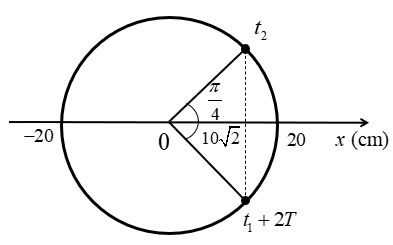
\includegraphics[scale=0.9]{../figs/VN12-PH-02-A-001-6-V2-1.jpg}
		\end{center}
		
		Dựa vào đường tròn lượng giác ta thấy sau $\dfrac{1}{4}T$ kể từ vị trí vật đang có li độ $x_1=10\sqrt{2}\,\text{cm}=\dfrac{A\sqrt{2}}{2}$ và chuyển động theo chiều dương, vật dao động đến vị trí  $x_1=10\sqrt{2}\,\text{cm}=\dfrac{A\sqrt{2}}{2}$ theo chiều âm với quãng đường đi được là
		\begin{equation*}
			s_2=2\left( A-\dfrac{A\sqrt{2}}{2}\right) =(2-\sqrt{2})A=(2-\sqrt{2})\cdot\SI{20}{\centi\meter}\approx\SI{11,7}{\centi\meter}.
		\end{equation*}
		
		Quãng đường vật đi được từ thời điểm $t_1=\SI{0,5}{\second}$ đến $t_2=\SI{5}{\second}$ là
		\begin{equation*}
			s=s_1+s_2=\SI{160}{\centi\meter}+ \SI{11,7}{\centi\meter}=\SI{171,7}{\centi\meter}.
		\end{equation*}
		
		\textbf{Đáp án: D.}
	}
	
	\viduii{3}{Một vật dao động theo phương trình $x=4\sqrt 2 \cos \left(5\pi t -\dfrac{3\pi}{4}\right)\ \text{cm}$. Quãng đường vật đi từ thời điểm $t_1 = \SI{0,1}{s}$ đến $t_2 =\SI{6}{s}$ là
		\begin{mcq}(4)
			\item $\SI{84,4}{cm}$.
			\item $\SI{333,8}{cm}$.
			\item $\SI{331,4}{cm}$.
			\item $\SI{337,5}{cm}$.
		\end{mcq}
	}
	{\begin{center}
			\textbf{Hướng dẫn giải}
		\end{center}
		
		Chu kỳ của dao động 
		\begin{equation*}
			T=\dfrac{2\pi}{\omega} = \SI{0,4}{s}.
		\end{equation*}
		\begin{itemize}
			\item Tại $t=\SI{0,1}{s}$ vật đi qua vị trí $x=\SI{4}{cm}$ theo chiều dương.
			\item Phân tích khoảng thời gian 
			\begin{equation*}
				\Delta t =t_2 -t_1  =\SI{5,9}{s}= \text{14,75}T.
			\end{equation*}
			\item Trong $\text{14,5}T$ đầu vật đi được quãng đường $14\cdot 4A +2A =58A$.
			\item Quãng đường vật đi được trong $\text{0,25}T$ còn lại là: 
			\begin{equation*}
				2A\left(A-\dfrac{\sqrt 2}{2}\right).
			\end{equation*}
		\end{itemize}
		$\Rightarrow$ Tổng quãng đường vật đi được là:
		\begin{equation*}
			S =58A + 2A\left(A-\dfrac{\sqrt 2}{2}\right) = \SI{331,4}{cm}.
		\end{equation*}
		
		\textbf{Đáp án: C.}
	}
\end{dang}
\begin{dang}{Quãng đường lớn nhất và nhỏ nhất\\ vật đi được trong khoảng thời gian $\Delta t$}
	\ppgiai{\textbf{Trường hợp $0<\Delta t<\dfrac{T}{2}$:}
		\begin{itemize}
			\item Quãng đường lớn nhất: Vật đi từ $\text{M}_1$ đến $\text{M}_2$ đối xứng qua trục sin:
			\begin{equation*}
				S_\text{max}=2A\sin\dfrac{\Delta \alpha}{2}=2A\sin\dfrac{\omega\Delta t}{2}.
			\end{equation*}
			\begin{center}
				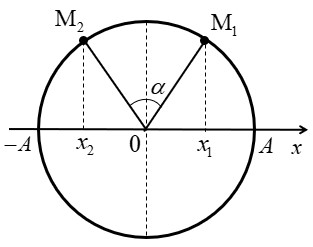
\includegraphics[scale=0.8]{../figs/VN12-PH-02-A-001-6-V2-2.jpg}
			\end{center}
			\item Quãng đường nhỏ nhất: Vật đi từ $\text{M}_1$ đến $\text{M}_2$ đối xứng qua trục cos:
			\begin{equation*}
				S_\text{min}=2A\left(1-\cos\dfrac{\Delta \alpha}{2}\right) =2A\left(1-\cos\dfrac{\omega\Delta t}{2}\right).
			\end{equation*}
			\begin{center}
				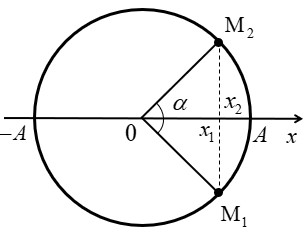
\includegraphics[scale=0.8]{../figs/VN12-PH-02-A-001-6-V2-3.jpg}
			\end{center}
		\end{itemize}
		
		\textbf{Trường hợp $\Delta t>\dfrac{T}{2},\ \Delta t=n\dfrac{T}{2}+\Delta t'\ \left( 0<\Delta t<\dfrac{T}{2}\right)$:}
		\begin{itemize}
			\item Quãng đường lớn nhất: Vật đi từ $\text{M}_1$ đến $\text{M}_2$ đối xứng qua trục sin:
			\begin{equation*}
				S_\text{max}=2nA+2A\sin\dfrac{\Delta \alpha}{2}=2nA+2A\sin\dfrac{\omega\Delta t'}{2}.
			\end{equation*}
			\item Quãng đường nhỏ nhất: Vật đi từ $\text{M}_1$ đến $\text{M}_2$ đối xứng qua trục cos:
			\begin{equation*}
				S_\text{min}=2nA+2A\left(1-\cos\dfrac{\Delta \alpha}{2}\right) =2nA+2A\left(1-\cos\dfrac{\omega\Delta t'}{2}\right).
			\end{equation*}
		\end{itemize}
	}
	\viduii{3}
	{
		Một vật dao động điều hòa với biên độ $A$ và chu kì $T$. Tìm quãng đường nhỏ nhất và lớn nhất mà vật đi được trong các khoảng thời gian $\dfrac{T}{6}$, $\dfrac{T}{4}$, $\dfrac{T}{3}$.
	}
	{\begin{center}
			\textbf{Hướng dẫn giải}
		\end{center}
		
		Góc mà vật quét được trong khoảng thời gian $\dfrac{T}{6}$ là
		\begin{equation*}
			\Delta\alpha=\omega\cdot\Delta t=\dfrac{2\pi}{T}\cdot\dfrac{T}{6}=\dfrac{\pi}{3}.
		\end{equation*}
		
		Góc mà vật quét được trong khoảng thời gian $\dfrac{T}{4}$ là
		\begin{equation*}
			\Delta\alpha=\omega\cdot\Delta t=\dfrac{2\pi}{T}\cdot\dfrac{T}{4}=\dfrac{\pi}{2}.
		\end{equation*}
		
		Góc mà vật quét được trong khoảng thời gian $\dfrac{T}{3}$ là
		\begin{equation*}
			\Delta\alpha=\omega\cdot\Delta t=\dfrac{2\pi}{T}\cdot\dfrac{T}{3}=\dfrac{2\pi}{3}.
		\end{equation*}
		
		Quãng đường nhỏ nhất mà vật đi được trong các khoảng thời gian $\dfrac{T}{6}$ là 
		\begin{equation*}
			S_\text{min}=2A\left(1-\cos\dfrac{\Delta \alpha}{2}\right)=2A\left(1-\cos\dfrac{\pi}{6}\right)=A(2-\sqrt{3}).
		\end{equation*}
		
		Quãng đường nhỏ nhất mà vật đi được trong các khoảng thời gian $\dfrac{T}{4}$ là 
		\begin{equation*}
			S_\text{min}=2A\left(1-\cos\dfrac{\Delta \alpha}{2}\right)=2A\left(1-\cos\dfrac{\pi}{4}\right)=A(2-\sqrt{2}).
		\end{equation*}
		
		Quãng đường nhỏ nhất mà vật đi được trong các khoảng thời gian $\dfrac{T}{3}$ là 
		\begin{equation*}
			S_\text{min}=2A\left(1-\cos\dfrac{\Delta \alpha}{2}\right)=2A\left(1-\cos\dfrac{\pi}{3}\right)=A.
		\end{equation*}
		
		Quãng đường lớn nhất mà vật đi được trong các khoảng thời gian $\dfrac{T}{6}$ là 
		\begin{equation*}
			S_\text{max}=2A\sin\dfrac{\Delta \alpha}{2}=2A\sin\dfrac{\pi}{6}=A.
		\end{equation*}
		
		Quãng đường lớn nhất mà vật đi được trong các khoảng thời gian $\dfrac{T}{4}$ là 
		\begin{equation*}
			S_\text{max}=2A\sin\dfrac{\Delta \alpha}{2}=2A\sin\dfrac{\pi}{4}=A\sqrt{2}.
		\end{equation*}
		
		Quãng đường lớn nhất mà vật đi được trong các khoảng thời gian $\dfrac{T}{3}$ là 
		\begin{equation*}
			S_\text{max}=2A\sin\dfrac{\Delta \alpha}{2}=2A\sin\dfrac{\pi}{3}=A\sqrt{3}.
		\end{equation*}
	}
	\viduii{3}
	{
		Một vật dao động điều hòa dọc theo trục O$x$, quanh vị trí cân bằng O với biên độ $A$ và chu kỳ $T$. Trong khoảng thời gian $\dfrac{T}{6}$, tỉ số quãng đường lớn nhất / nhỏ nhất mà vật có thể đi được là
		\begin{mcq}(4)
			\item $2$.
			\item $2+\sqrt 3$.
			\item $2+\sqrt 2$.
			\item $3$. 
		\end{mcq}
	}
	{
		\begin{center}
			\textbf{Hướng dẫn giải}
		\end{center}
		
		Ta có:
		\begin{equation*}
			\Delta t =\dfrac{T}{6}.
		\end{equation*}
		Tỉ số quãng đường lớn nhất / nhỏ nhất mà vật có thể đi được là
		\begin{equation*}
			\dfrac{S_\text{max}}{S_\text{min}} = \dfrac{2A \sin \dfrac{\pi \Delta t}{T}}{2A\left (1-\cos \dfrac{\pi \Delta t }{T}\right)}=\dfrac{2A\sin \dfrac{\pi}{6}}{2A\left(1-\cos \dfrac{\pi}{6}\right)} =2+\sqrt 3.
		\end{equation*}
		
		\textbf{Đáp án: B.}
	}
\end{dang}
\begin{dang}{Sử dụng được phương trình dao động\\ và đường tròn lượng giác\\ để xác định thời gian}
	\viduii{3}{Một vật dao động điều hòa trên trục $\text{O}x$ với phương trình
		$x=5\cos\left( 4\pi t-\dfrac{\pi}{3}\right)$ ($x$ tính bằng cm, $t$ tính bằng s). Khoảng thời gian ngắn nhất để vật đi từ li độ $x_1=\SI{-2,5}{\centi\meter}$ đến li độ $x_2=2,5\sqrt{3}\,\text{cm}$ là
		\begin{mcq}(4)
			\item $\dfrac{1}{8}\,\text{s}$.
			\item $\dfrac{1}{4}\,\text{s}$.
			\item $\dfrac{1}{6}\,\text{s}$.
			\item $\dfrac{1}{2}\,\text{s}$.
		\end{mcq}
	}
	{\begin{center}
			\textbf{Hướng dẫn giải}
		\end{center}
		
		\begin{center}
			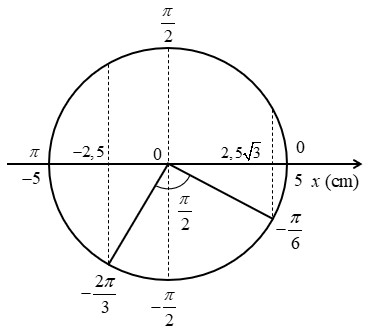
\includegraphics[scale=0.8]{../figs/VN12-PH-02-A-001-7-V2-2.jpg}
		\end{center}
		
		Dựa vào đường tròn lượng giác ta tính được góc quay $\Delta\alpha=\dfrac{\pi}{2}\,\text{rad}$.
		
		Thời gian ngắn nhất để vật đi từ vị trí có li độ $x_1=\SI{-2,5}{\centi\meter}$ đến li độ $x_2=2,5\sqrt{3}\,\text{cm}$ là
		\begin{equation*}
			\Delta t=\dfrac{\Delta\alpha}{\omega}=\dfrac{\dfrac{\pi}{2}\,\text{rad}}{4\pi\,\text{rad/s}}=\SI{0,125}{\second}.
		\end{equation*}
		
		\manatip{Vì $x_1=-\dfrac{A}{2}$ và $x_2 = \dfrac{A\sqrt{3}}{2}$ nên ta có thể tính nhanh $\Delta t = \dfrac{T}{12}+\dfrac{T}{6}=\dfrac{T}{4}=\dfrac{1}{8}\ \text s$.}
		
		\textbf{Đáp án: A.}
	}
	\viduii{3}{Một vật dao động điều hòa theo phương trình $x=4\cos \left(20\pi t -\dfrac{\pi}{2}\right)\ \text{cm}$. Thời gian ngắn nhất để vật đi từ vị trí có li độ $x_1=\SI{2}{cm}$ đến li độ $x_2=\SI{4}{cm}$ bằng
		\begin{mcq}(4)
			\item $\dfrac{1}{80}\ \text{s}$.
			\item $\dfrac{1}{60}\ \text{s}$.
			\item $\dfrac{1}{120}\ \text{s}$.
			\item $\dfrac{1}{40}\ \text{s}$.
		\end{mcq}
	}
	{\begin{center}
			\textbf{Hướng dẫn giải}
		\end{center}
		
		Chu kỳ của vật dao động:
		\begin{equation*}
			T =\dfrac{2\pi}{\omega} =\SI{0,1}{s}.
		\end{equation*}
		\begin{center}
			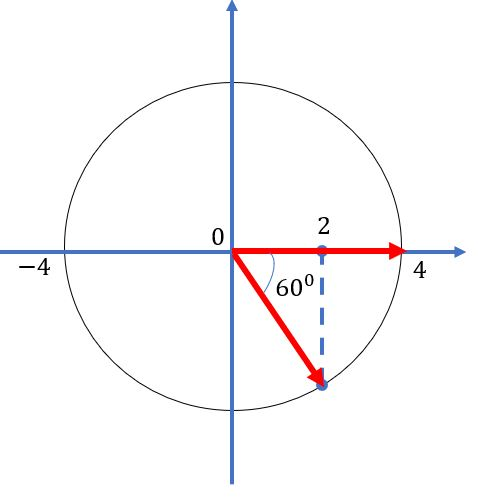
\includegraphics[scale=0.6]{../figs/VN12-PH-02-A-001-7-V2-3.jpg}
		\end{center}
		Thời gian ngắn nhất để vật đi từ vị trí có li độ $x_1 = \SI{2}{cm}$ đến li độ $x_2 =\SI{4}{cm}$ bằng
		\begin{equation*}
			\Delta t =\dfrac{T}{6}= \dfrac{1}{60}\ \text{s}.
		\end{equation*}
		
		\textbf{Đáp án: B.}
	}
	
\end{dang}
\begin{dang}{Xác định được thời gian ngắn nhất\\ và dài nhất để vật đi hết quãng đường}
	\ppgiai{
		Vật dao động điều hòa có tốc độ càng lớn khi vật càng gần vị trí cân bằng và tốc độ càng nhỏ khi vật càng gần vị trí biên.
		
		\begin{enumerate}[label=\alph*)]
			\item Nếu $S<2A$
			
			Thời gian ngắn nhất vật đi được quãng đường $S$ là
			\begin{equation*}
				S=2A\sin\dfrac{\Delta \alpha_\text{min}}{2}=2A\sin\dfrac{\omega\Delta t_\text{min}}{2}.
			\end{equation*}
			Thời gian dài nhất vật đi được quãng đường $S$ là
			\begin{equation*}
				S=2A\left(1-\cos\dfrac{\Delta \alpha_\text{max}}{2}\right) =2A\left(1-\cos\dfrac{\omega\Delta t_\text{max}}{2}\right).
			\end{equation*}
			\item Nếu $S>2A$
			
			Ta phân tích quãng đường như sau:
			\begin{equation*}
				S=n2A+S'.
			\end{equation*}
			
			Thời gian vật đi được quãng đường $S$ là
			\begin{equation*}
				\Delta t=n\dfrac{T}{2}+\Delta t'.
			\end{equation*}
			
			Khi đó ta tìm $\Delta t'_\text{min}$ và $\Delta t'_\text{max}$ như trường hợp a).
		\end{enumerate}	
	}
	\viduii{3}
	{
		Một vật nhỏ dao động điều hòa với bên độ $A$ và tần số góc $\omega$. Thời gian ngắn nhất để vật đi được quãng đường có độ dài $A\sqrt{3}$ là
		\begin{mcq}(4)
			\item $\dfrac{\pi}{6\omega}$.
			\item $\dfrac{\pi}{12\omega}$.
			\item $\dfrac{1}{6\omega}$.
			\item $\dfrac{2\pi}{3\omega}$.
		\end{mcq}
	}
	{\begin{center}
			\textbf{Hướng dẫn giải}
		\end{center}
		
		Thời gian ngắn nhất vật đi được quãng đường $S=A\sqrt{3}$ là
		\begin{equation*}
			S=2A\sin\dfrac{\omega\Delta t_\text{min}}{2}\Rightarrow \Delta t_\text{min}=\dfrac{2}{\omega}\cdot \arcsin \dfrac{S}{2A}=\dfrac{2}{\omega}\cdot \arcsin \dfrac{A\sqrt{3}}{2A}=\dfrac{2\pi}{3\omega}.
		\end{equation*}
		
		\textbf{Đáp án: D.}
	}
	\viduii{3}
	{
		Một vật dao động điều hòa với biên độ $A$ và tần số $f$. Thời gian ngắn nhất để vật đi được quãng đường có độ dài $3A$ là
		\begin{mcq}(4)
			\item $\dfrac{3}{4f}$.
			\item $\dfrac{2}{3f}$.
			\item $\dfrac{5}{6f}$.
			\item $\dfrac{5}{4f}$.
		\end{mcq}
	}
	{
		\begin{center}
			\textbf{Hướng dẫn giải}
		\end{center}
		
		Ta phân tích quãng đường như sau:
		\begin{equation*}
			3A=2A+A.
		\end{equation*}
		
		Suy ra thời gian ngắn nhất vật đi được quãng đường $S=3A$ là
		\begin{equation*}
			\Delta t=\dfrac{T}{2}+\Delta t';
		\end{equation*}
		với $\Delta t'$ là thời gian ngắn nhất để vật đi hết quãng đường $A$.
		
		Thời gian ngắn nhất vật đi được quãng đường $S'=A$ là
		\begin{equation*}
			S'=2A\sin\dfrac{\omega\Delta t_\text{min}}{2}\Rightarrow \Delta t_\text{min}=\dfrac{2}{\omega}\cdot \arcsin \dfrac{S'}{2A}=\dfrac{2}{\omega}\cdot \arcsin \dfrac{A}{2A}=\dfrac{\pi}{3\omega}=\dfrac{T}{6}.
		\end{equation*}
		
		Vậy thời gian ngắn nhất vật đi được quãng đường $S=3A$ là
		\begin{equation*}
			\Delta t=\dfrac{T}{2}+\dfrac{T}{6}=\dfrac{2T}{3}=\dfrac{2}{3f}.
		\end{equation*}
		
		\textbf{Đáp án: B.}
	}
\end{dang}